\documentclass[12 pt]{article}
\usepackage[T1]{fontenc}
\usepackage[utf8]{luainputenc}
\usepackage{amssymb}
\usepackage{amsmath}
\usepackage[T1,T2A]{fontenc}
\usepackage[utf8]{inputenc}
\usepackage{tikz}

\begin{document}

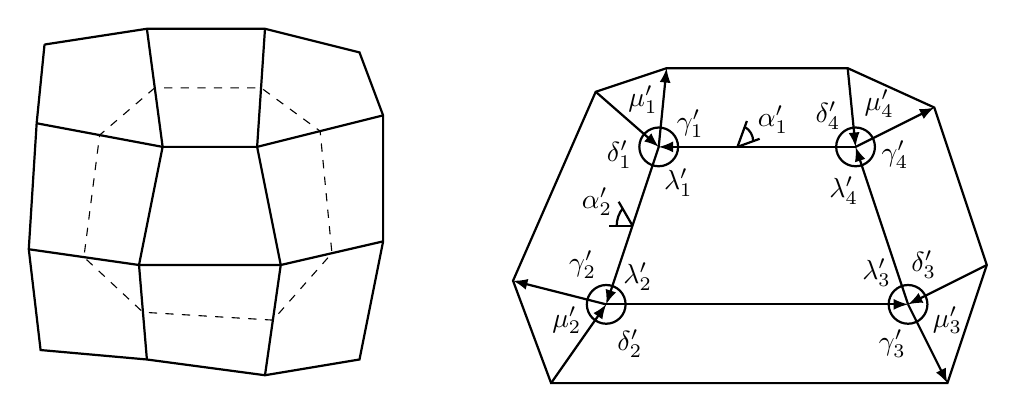
\begin{tikzpicture}[>=latex]

       \coordinate (A1) at (0.2, 4.3);
       \coordinate (A2) at (0.1, 3.3);
       \coordinate (A3) at (0, 1.7);
       \coordinate (A4) at (0.15, 0.42);
       \coordinate (A5) at (1.5, 0.3);
       \coordinate (A6) at (3, 0.1);
       \coordinate (A7) at (4.2, 0.3);
       \coordinate (A8) at (4.5, 1.8);
       \coordinate (A9) at (4.5, 3.4);
       \coordinate (A10) at (4.2, 4.2);
       \coordinate (A11) at (3, 4.5);
       \coordinate (A12) at (1.5, 4.5);

       \coordinate (B1) at (1.7, 3);
       \coordinate (B2) at (1.4, 1.5);
       \coordinate (B3) at (3.2, 1.5);
       \coordinate (B4) at (2.9, 3);

       \coordinate (C1) at (1.6,3.75);
       \coordinate (C2) at (0.9,3.15);
       \coordinate (C3) at (0.7,1.6);
       \coordinate (C4) at (1.45,0.9);
       \coordinate (C5) at (3.1,0.8);
       \coordinate (C6) at (3.85,1.65);
       \coordinate (C7) at (3.7,3.2);
       \coordinate (C8) at (2.95,3.75);

       \draw[thick] (A1) -- (A2) -- (A3) --(A4) --(A5) --(A6) --(A7) --(A8) --(A9) --(A10) --(A11) --(A12) --(A1);
       \draw[thick] (B1) -- (B2) -- (B3) --(B4) --(B1);
       \draw[dashed] (C1) -- (C2) -- (C3) --(C4) --(C5) --(C6) --(C7) --(C8) --(C1);

       \draw[thick] (B1) -- (A12);
       \draw[thick] (B1) -- (A2);

       \draw[thick] (B2) -- (A3);
       \draw[thick] (B2) -- (A5);

       \draw[thick] (B3) -- (A6);
       \draw[thick] (B3) -- (A8);

       \draw[thick] (B4) -- (A9);
       \draw[thick] (B4) -- (A11);


       \coordinate (a3) at (11.166667, 1);
       \coordinate (a2) at (7.333333, 1);
       \coordinate (a1) at (8, 3);
       \coordinate (a4) at (10.5, 3);
       \coordinate (b3) at (12.166667, 1.5);
       \coordinate (c3) at (11.666667, 0);
       \coordinate (b2) at (6.633333, 0);
       \coordinate (c2) at (6.15, 1.3);
       \coordinate (b1) at (7.2, 3.7);
       \coordinate (c1) at (8.1, 4);
       \coordinate (b4) at (10.4, 4);
       \coordinate (c4) at (11.5, 3.5);





       \draw[thick] (b3) -- (c3) -- (b2) -- (c2) -- (b1) -- (c1) -- (b4) -- (c4) -- cycle;

       \draw[thick,<-] (a3) -- (a2);
       \draw[thick,<-] (a2) -- (a1);
       \draw[thick,<-] (a1) -- (a4);
       \draw[thick,<-] (a4) -- (a3);

       \draw[thick,<-] (a3) -- (b3);
       \draw[thick,->] (a3) -- (c3);

       \draw[thick,<-] (a2) -- (b2);
       \draw[thick,->] (a2) -- (c2);

       \draw[thick,<-] (a1) -- (b1);
       \draw[thick,->] (a1) -- (c1);

       \draw[thick,<-] (a4) -- (b4);
       \draw[thick,->] (a4) -- (c4);






       \draw[thick] (a3) circle (7pt);
       \draw (a3)+(-0.4, 0.4) node {$\lambda_3'$};
       \draw (a3)+(0.2, 0.5) node {$\delta_3'$};
       \draw (a3)+(0.5, -0.2) node {$\mu_3'$};
       \draw (a3)+(-0.2, -0.5) node {$\gamma_3'$};

       \draw[thick] (a2) circle (7pt);
       \draw (a2) + (0.4, 0.35) node {$\lambda_2'$};
       \draw (a2) + (-0.3, 0.5) node {$\gamma_2'$};
       \draw (a2) + (-0.5, -0.2) node {$\mu_2'$};
       \draw (a2) + (0.3, -0.5) node {$\delta_2'$};

       \draw[thick] (a1) circle (7pt);
       \draw (a1) + (0.25, -0.45) node {$\lambda_1'$};
       \draw (a1) + (0.4, 0.3) node {$\gamma_1'$};
       \draw (a1) + (-0.2, 0.6) node {$\mu_1'$};
       \draw (a1) + (-0.5, -0.1) node {$\delta_1'$};

       \draw[thick] (a4) circle (7pt);
       \draw (a4) + (-0.15, -0.55) node {$\lambda_4'$};
       \draw (a4) + (0.3, 0.55) node {$\mu_4'$};
       \draw (a4) + (-0.35, 0.4) node {$\delta_4'$};
       \draw (a4) + (0.5, -0.1) node {$\gamma_4'$};

        \coordinate (alpha1) at (9, 3);
       \draw[thick, rotate around = {-20:(alpha1)}] (alpha1) -- + (0, 0.35);
       \draw[thick, rotate around = {20:(alpha1)}] (alpha1) -- + (0.3, 0);
       \draw[thick] (alpha1) + (0.2, .07) arc (0:60:6pt);
       \draw (alpha1) + (.45, .35) node {$\alpha_1'$};

       \coordinate (psi3) at (7.66667, 2);
       \draw[thick, , rotate around = {30:(psi3)}] (psi3) -- + (0, 0.35);
       \draw[thick, , rotate around = {0:(psi3)}] (psi3) -- + (-0.3, 0);
       \draw[thick] (psi3) + (-0.2, 0) arc (180:141:10pt);
       \draw (psi3) + (-0.45, 0.3) node {$\alpha_2'$};

   \end{tikzpicture}

\end{document}